\documentclass[usenames,dvipsnames,11pt,pdf,utf8,russian,aspectratio=169]{beamer}
\usepackage{cmap}
\usepackage[T2A]{fontenc}
\usepackage[english,russian]{babel}
\usepackage{subfig}
\usepackage{color}
\usepackage{multicol}
\usepackage{appendixnumberbeamer}
\usepackage{multicol}

\DeclareMathOperator*{\argmin}{arg\,min}

\DeclareMathOperator*{\argmax}{arg\,max}
%
% Choose how your presentation looks.
%
% For more themes, color themes and font themes, see:
% http://deic.uab.es/~iblanes/beamer_gallery/index_by_theme.html
%
\mode<presentation>
{
  \usetheme{Boadilla}      % or try Darmstadt, Madrid, Warsaw, ...
  \usecolortheme{seagull} % or try albatross, beaver, crane, ..

  \usefonttheme{structurebold}  % or try serif, structurebold, ...
  \setbeamertemplate{navigation symbols}{}
  \setbeamertemplate{caption}[numbered]
} 

\captionsetup[subfloat]{labelformat=empty}
\title[Выбор структуры модели]{Байесовский выбор\\ наиболее правдоподобной структуры\\ модели глубокого обучения}
\author{О.\,Ю.\,Бахтеев}


\institute[МФТИ]{Научный руководитель: д.ф.-м.н. В.В. Стрижов\\Московский физико-технический институт (государственный университет)}     
%\institute[МФТИ]{Московский Физико-Технический Институт (Государственный Университет)}
\date[2018]{Интеллектуализация обработки информации\\ ИОИ-2018 \\11.10.2018\\}
\begin{document}

\begin{frame}
  \titlepage
\end{frame}



\begin{frame}{Выбор  структуры модели глубокого обучения}

\textbf{Цель работы:}\\
Развитие теории байесовского выбора модели и исследование свойств методов выбора моделей глубокого обучения.\\
\textbf{Задачи:}
\begin{itemize}
\item Предложить алгоритм оптимизации параметров, гиперпараметров и структурных параметров моделей глубокого обучения.
\item Предложить метод выбора модели наиболее правдоподобной структуры.
\item Исследовать свойства оптимизационных алгоритмов выбора модели.
\end{itemize}
\textbf{Основные проблемы}
\begin{itemize}
\item Многоэкстремальность задачи оптимизации параметров модели.
\item Вычислительная сложность оптимизации.
\item Большое число параметров и гиперпараметров.
\end{itemize}

\end{frame}


\begin{frame}    
                                                                                                                        
\frametitle{Проблемы оптимизации моделей глубокого обучения}                                                                                                          
Правдоподобие моделей с избыточным количеством параметров не меняется при удалении параметров.                                                       
\begin{figure}[h]                                                                                                                               
\centering                                                                                                                                      
\subfloat[Избыточность параметров модели]{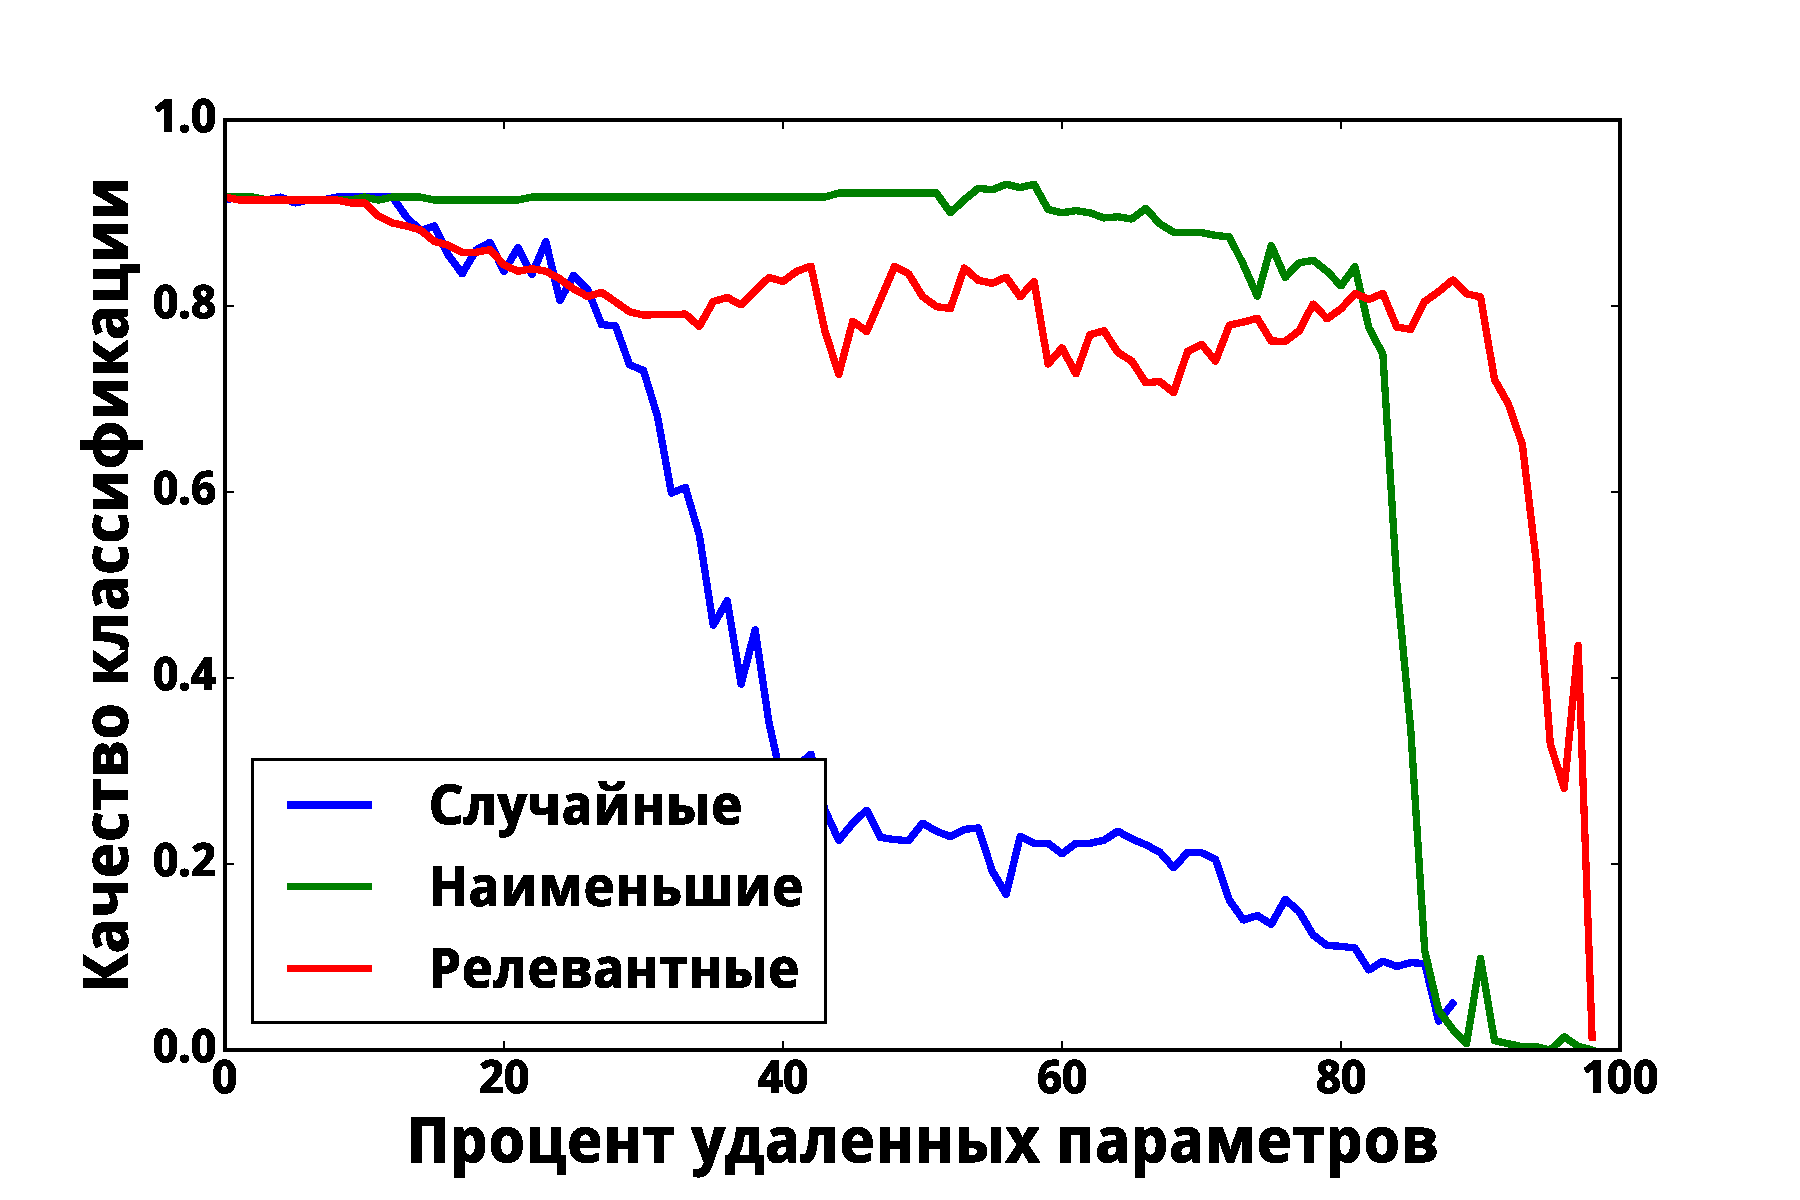
\includegraphics[width=0.45\textwidth]{./slide_plots/pruning.pdf}}                                          
\subfloat[Неустойчивость модели]{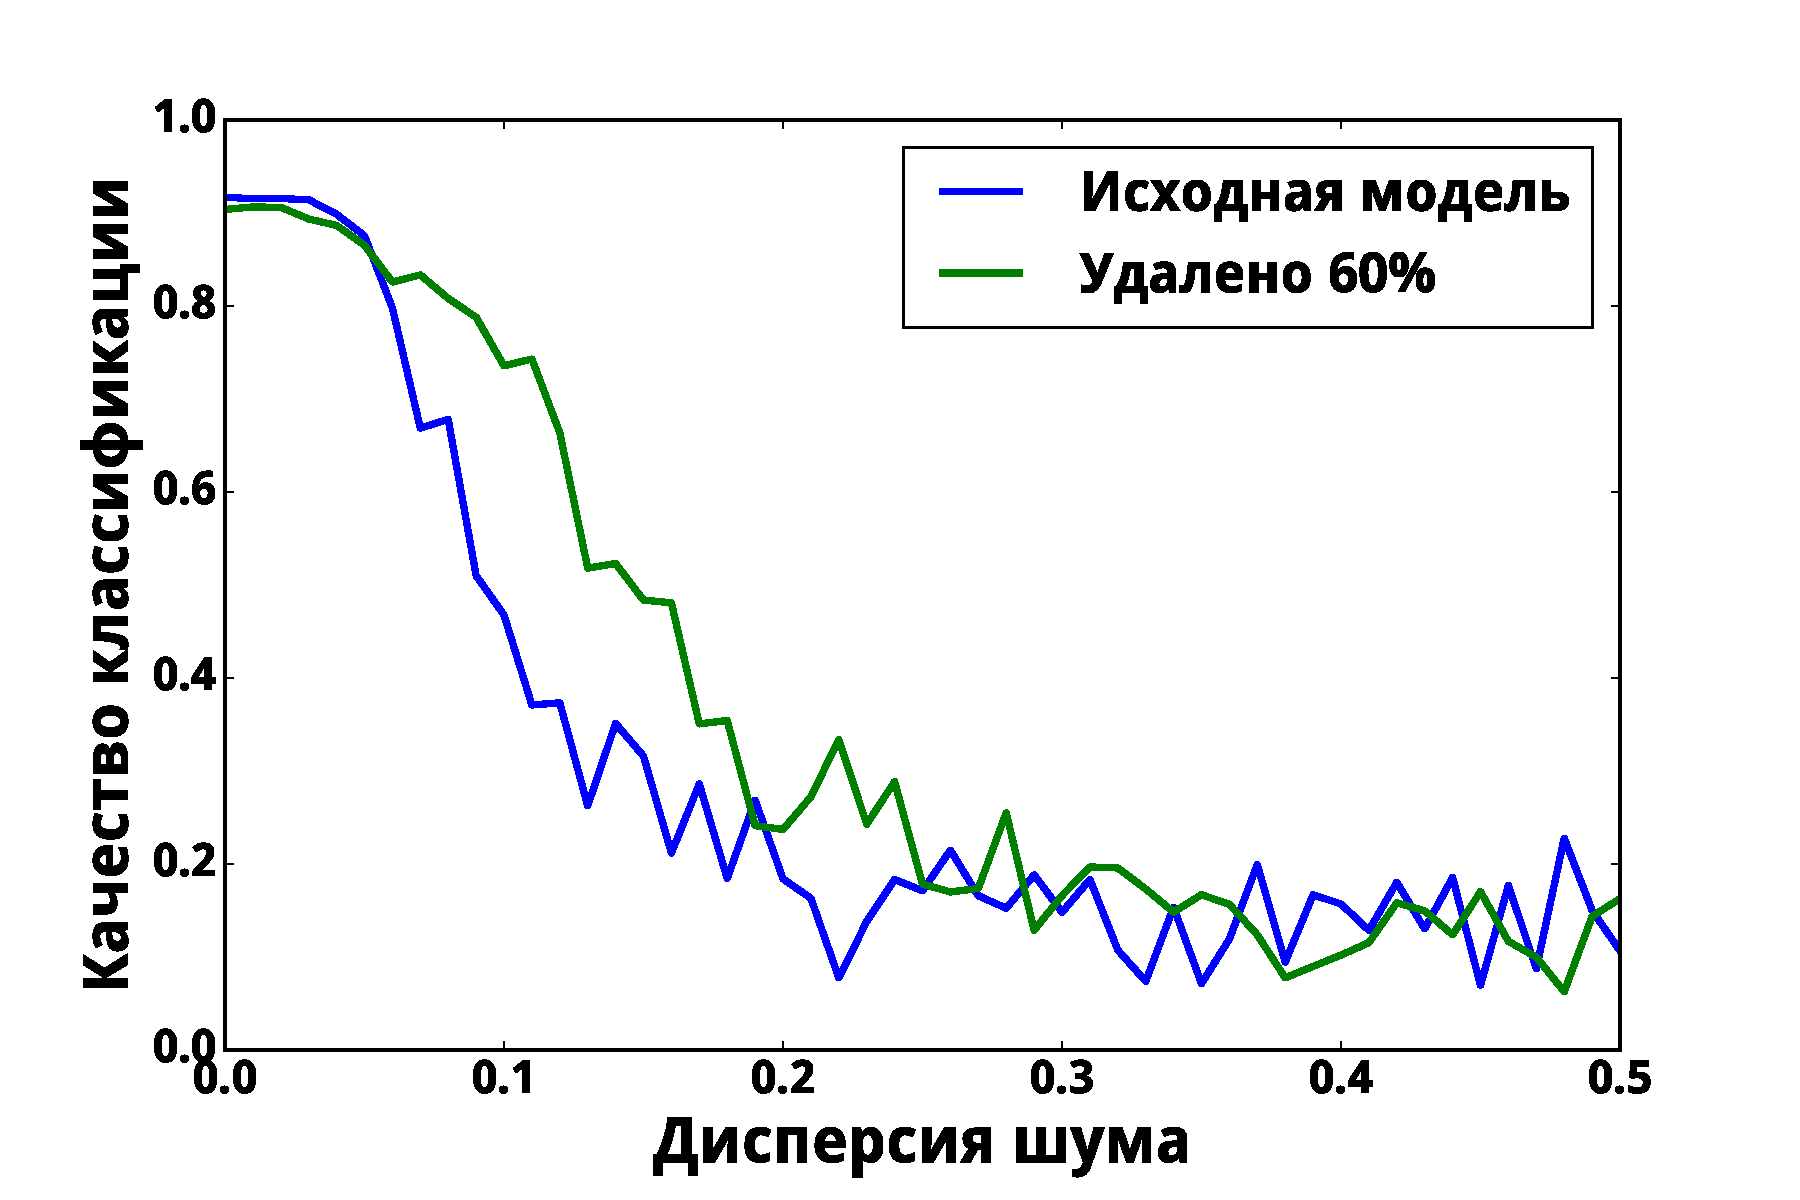
\includegraphics[width=0.45\textwidth]{./slide_plots/noise.pdf}}                                                     
\end{figure}                                                                                                   
\textcolor{gray}{Глубокое обучение предполагает оптимизацию моделей с заведомо избыточной сложностью.}  
                                                                                                                                             
\end{frame}    

\begin{frame}{Задача выбора структуры модели}

Однослойная нейросеть:
\[
    \mathbf{f}(\mathbf{x}) = \text{softmax}\left(\mathbf{W}_0^\text{T}\mathbf{f}_1(\mathbf{x})\right), \quad f(\mathbf{x}): \mathbb{R}^n \to [0,1]^{|\mathbb{Y}|}, \quad \mathbf{x} \in \mathbb{R}^n.
\]
\[
\]
\[
{f}_1(\mathbf{x}) = {\gamma}_{0,1}^{1}\mathbf{g}_{0,1}^{1}(\mathbf{x})+\dots+{\gamma}_{0,1}^{K}\mathbf{g}_{0,1}^{K}(\mathbf{x})= {\gamma}_{0,1}^{1}\boldsymbol{\sigma}(\mathbf{W}_1^\text{T}\mathbf{x}) + \dots +  {\gamma}_{0,1}^{K}\boldsymbol{\sigma}(\mathbf{W}_K^\text{T}\mathbf{x}),
\]
где $\mathbf{W} = [\mathbf{W}_0,\mathbf{W}_1, \dots, \mathbf{W}_K]^\text{T}$ --- матрицы параметров, $\{\mathbf{g}^{i}_{0,1}\}_{i=1}^K$ --- базовые функции скрытого слоя нейросети.~\\~\\

\textbf{Структурные параметры:}  $\boldsymbol{\Gamma} = [\boldsymbol{\gamma}_{0,1}]$.\\
\textbf{Структура модели} определяется вершиной $K$-мерного симплекса.
    
\end{frame}

\begin{frame}{Задача выбора структуры модели: два скрытых слоя}
Двухслойная нейросеть:
\[
    \mathbf{f}(\mathbf{x}) = \text{softmax}\left(\mathbf{W}^\text{T}\textcolor{red}{\mathbf{f}_2}(\mathbf{x})\right), \quad f(\mathbf{x}): \mathbb{R}^n \to [0,1]^{|\mathbb{Y}|}, \quad \mathbf{x} \in \mathbb{R}^n.
\]
\[
\textcolor{red}{
\mathbf{f}_2(\mathbf{x}) = {\gamma}_{1,2}^{1}\mathbf{g}_{1,2}^{1}(\mathbf{f}_1(\mathbf{x}))+\dots+{\gamma}_{1,2}^{K}\mathbf{g}_{1,2}^{K}(\mathbf{f}_1(\mathbf{x}))= {\gamma}_{1,2}^{1}\boldsymbol{\sigma}(\mathbf{W}_{K+1}^\text{T}\mathbf{f}_1(\mathbf{x})) + \dots +  {\gamma}_{1,2}^{K}\boldsymbol{\sigma}(\mathbf{W}_{2K}^\text{T}\mathbf{f}_1(\mathbf{x})),}
\]
\[
\mathbf{f}_1(\mathbf{x}) = {\gamma}_{0,1}^{1}\mathbf{g}_{0,1}^{1}(\mathbf{x})+\dots+{\gamma}_{0,1}^{K}\mathbf{g}_{0,1}^{K}(\mathbf{x})= {\gamma}_{0,1}^{1}\boldsymbol{\sigma}(\mathbf{W}_1^\text{T}\mathbf{x}) + \dots +  {\gamma}_{0,1}^{K}\boldsymbol{\sigma}(\mathbf{W}_K^\text{T}\mathbf{x}),
\]

где $\mathbf{W} = [\mathbf{W}_0,\textcolor{red}{\mathbf{W}_1, \dots, \mathbf{W}_{2K}}]^{\text{T}}$ --- матрицы параметров, $\{\mathbf{g}^{i}_{0,1}, \textcolor{red}{\mathbf{g}^{i}_{1,2}\}_{i=1}^K}$ --- базовые функции скрытых слоев нейросети.~\\~\\

\textbf{Структурные параметры:} $\boldsymbol{\Gamma} = [\boldsymbol{\gamma}_{0,1}, \textcolor{red}{\boldsymbol{\gamma}_{1,2}}]$.\\
\textbf{Структура модели} определяется вершинами \textcolor{red}{двух} $K$-мерных симплексов.
\end{frame}
        
\iffalse
\begin{frame}{}
Картинка: связь параметров со структурой.
\end{frame}
\fi

\begin{frame}{Исследование основывается на следующих работах}
\begin{itemize}
\item Graves A. Practical variational inference for neural networks //Advances in Neural Information Processing Systems. – 2011
\item  Maclaurin D., Duvenaud D., Adams R. Gradient-based hyperparameter optimization through reversible learning //International Conference on Machine Learning. – 2015.
\item Hanxiao L. et al., DARTS: Differentiable Architecture Search //  arXiv preprint:1806.09055, - 2018.
\item О. Ю. Бахтеев, В. В. Стрижов. Выбор моделей глубокого обучения субоптимальной сложности  //Автоматика и телемеханика, 2018.
\end{itemize}
\end{frame}


\begin{frame}{Графовое представление модели глубокого обучения}
\begin{block}{Определение}
Задан граф $V,E$. \\
Для каждого ребра $(j,k) \in E$ определен вектор \textbf{базовых функций} $\mathbf{g}_{j,k}$ мощностью $K_{j,k}$.\\
Граф $V, E$ со множеством функций $\{\mathbf{g}_{j,k}\}_{(j,k) \in E}$ называется \textbf{семейством моделей}, если функция, задаваемая рекурсивно как 
\[
    \mathbf{f}_j(\mathbf{x}) = \sum_{k \in \text{Adj}(v_j)} \langle \boldsymbol{\gamma}_{j,k}, \mathbf{g}_{j,k} \rangle (\mathbf{f}_{k}(\mathbf{x})), \quad     \mathbf{f}_0(\mathbf{x}) = \mathbf{x},
\]
является непрерывной дифференцируемой по параметрам функцией из $\mathbb{R}^n$ во множество $\mathbb{Y}$ при любых значениях векторов $\boldsymbol{\gamma}$.
\end{block}
\textbf{Модель} задается параметрами подмоделей $\{\mathbf{f}_j\}_{j=1}^{|V|}$ и структурными параметрами  $\boldsymbol{\gamma}$.\\
\textbf{Параметры модели}  $\mathbf{W}$ ---  конкатенация параметров всех подмоделей $\{\mathbf{f}_j\}_{j=1}^{|V|}$.\\
\textbf{Структура модели}  $\boldsymbol{\Gamma}$ --- конкатенация структурных параметров $\boldsymbol{\gamma}$.
\end{frame}




\begin{frame}
\frametitle{Эксплуатационные критерии качества модели}

\textbf{Точность} $S(\mathbf{W}, \boldsymbol{\Gamma})$ модели $\mathbf{f}(\mathbf{x})$ --- величина ошибки на контрольной выборке.
~\\
~\\
\textbf{Устойчивость} $\eta(\mathbf{{W}})$ модели $\mathbf{f}(\mathbf{x})$ --- число обусловленности матрицы $\mathbf{A}$:
$$\eta(\mathbf{{W}})=\frac{\lambda_{\max}}{\lambda_{\min}} \quad\text{при гипотезе } 	\mathbf{W} \sim \mathcal{N}(\mathbf{0},\mathbf{A}^{-1}),$$  $\lambda_{\max}$ --- максимальное, а $\lambda_{\min}$ --- минимальное собственные числа матрицы $\mathbf{A}$.





\end{frame}

\begin{frame}{Статистические критерии качества модели}
\small


\textbf{Параметрическая сложность} --- наименьшая дивергенция между априорным распределением параметров и апостериорным распределением параметров:
\[
    C_\text{param} = \min_{\mathbf{A}, \mathbf{m}} \text{D}_\text{KL}(p(\mathbf{W}, \boldsymbol{\Gamma}|\mathbf{y}, \mathbf{X})||p(\mathbf{W}, \boldsymbol{\Gamma}||\mathbf{A}, \mathbf{m})).
\]
где $\mathbf{m}$ --- гиперпараметры априорного распределения структуры модели.

\textcolor{red}{\textbf{TODO: bits-back!\\}}

\textbf{Структурная сложность модели} --- энтропия апостериорного распределения структуры модели:
\[
    C_\text{struct} = -\mathsf{E}_{p} \text{log}~p(\boldsymbol{\Gamma}|\mathbf{y}, \mathbf{X}).
\]

\textcolor{red}{В данной работе предлагается метод оптимизации модели, учитывающий все перечисленные критерии качества модели. }
\end{frame}


\begin{frame}{Правдоподобие как статистическая сложность}  
\small
\textbf{Статистическая сложность} модели $\mathbf{f}$:
\[
	\text{MDL}(\mathbf{y},\mathbf{f}) = -\text{log}~p(\mathbf{f}) - \text{log}~\bigl(p(\mathbf{y}|\mathbf{X}, \mathbf{f})\delta\mathfrak{D})\bigr),
\]
где $\delta\mathfrak{D}$ --- допустимая точность передачи информации о выборке $\mathfrak{D}$.

\textbf{Правдоподобия модели}:                                      
\[                                                                                                                                              
        p(\mathbf{y}|\mathbf{X}) = \int_{\mathbf{W}, \boldsymbol{\Gamma} } \textcolor{red}{p(\mathbf{y}|\mathbf{X},\mathbf{W},  \boldsymbol{\Gamma})} \textcolor{blue}{p(\mathbf{W}, \boldsymbol{\Gamma}) d\mathbf{W}d{\boldsymbol{\Gamma}}}.                         
\]       


\begin{figure}
\vspace{-0.5cm}
  \centering
 \subfloat[Схема выбора модели по правдоподобию]{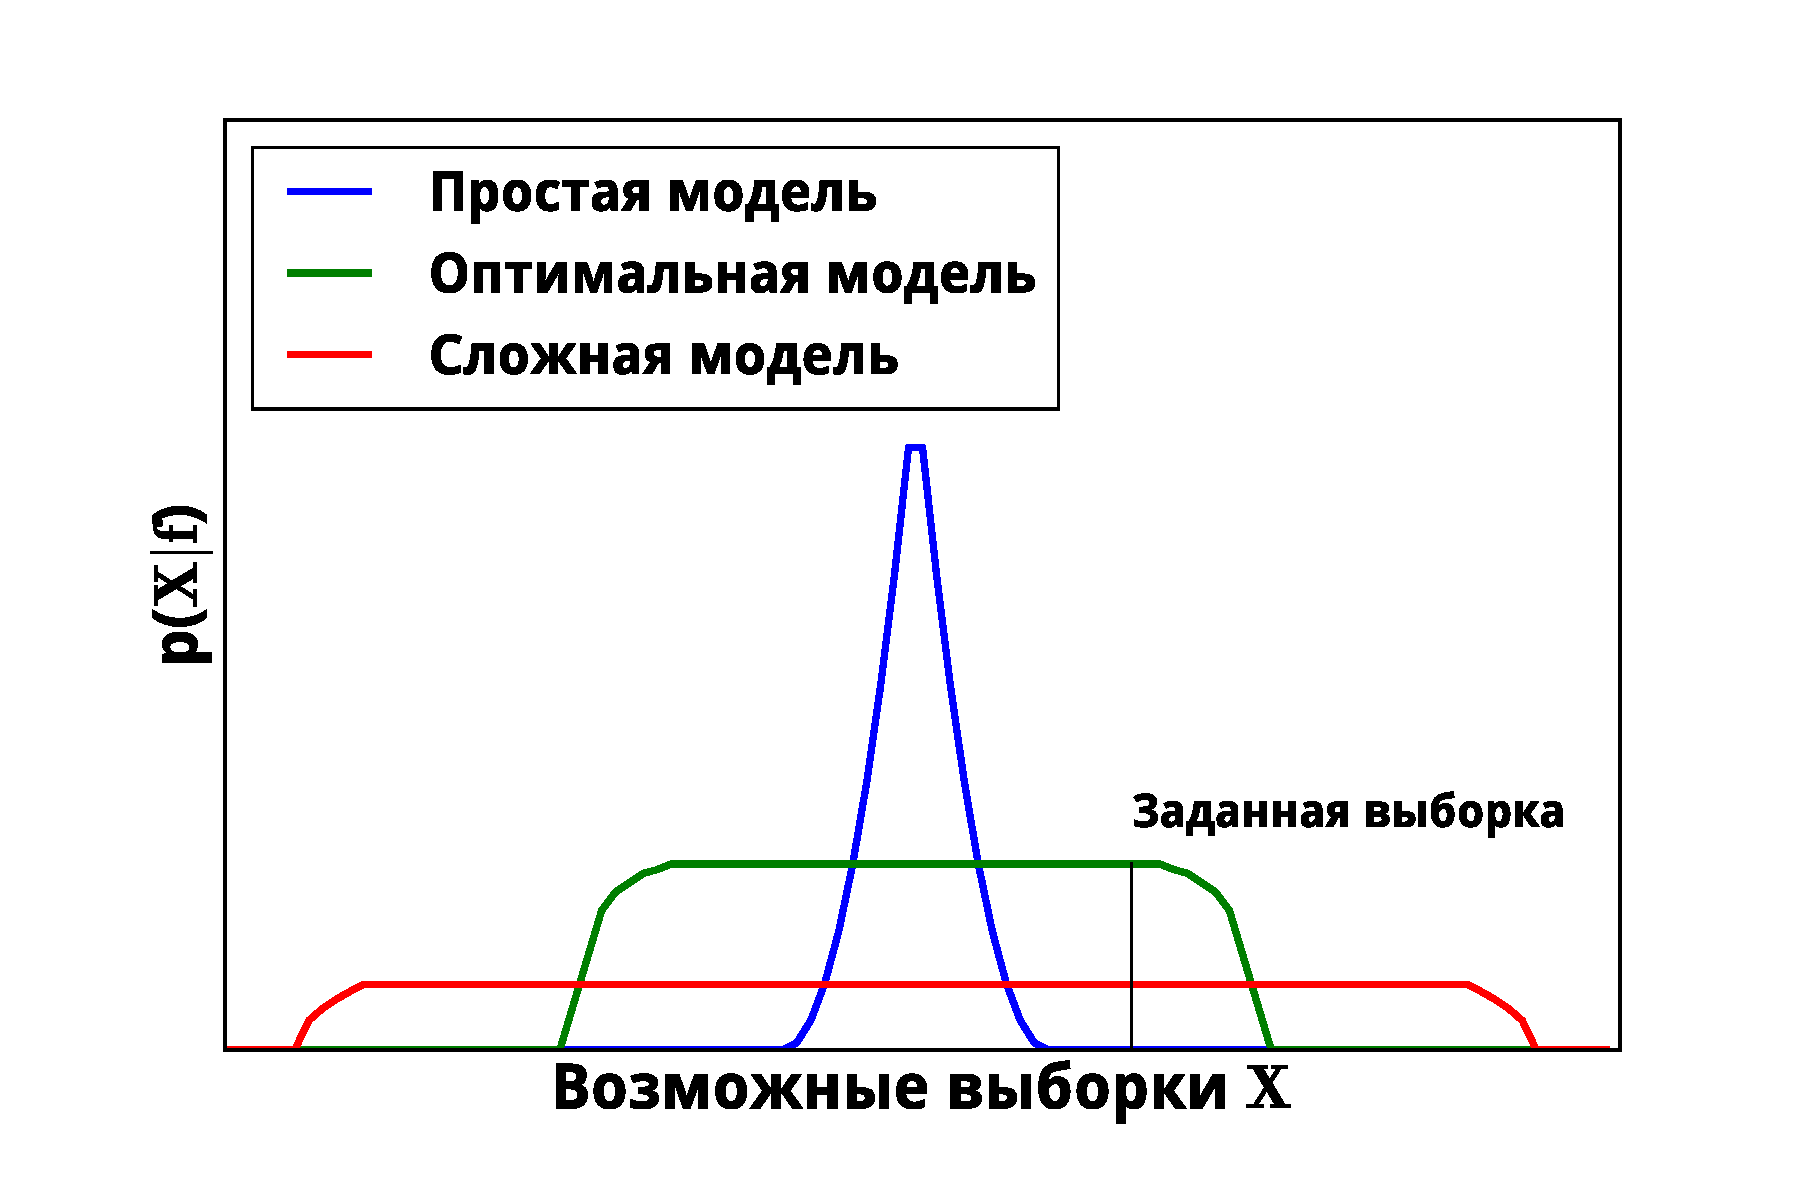
\includegraphics[width=0.35\textwidth]{slide_plots/evidence.pdf}} 
 \subfloat[Пример: полиномы]{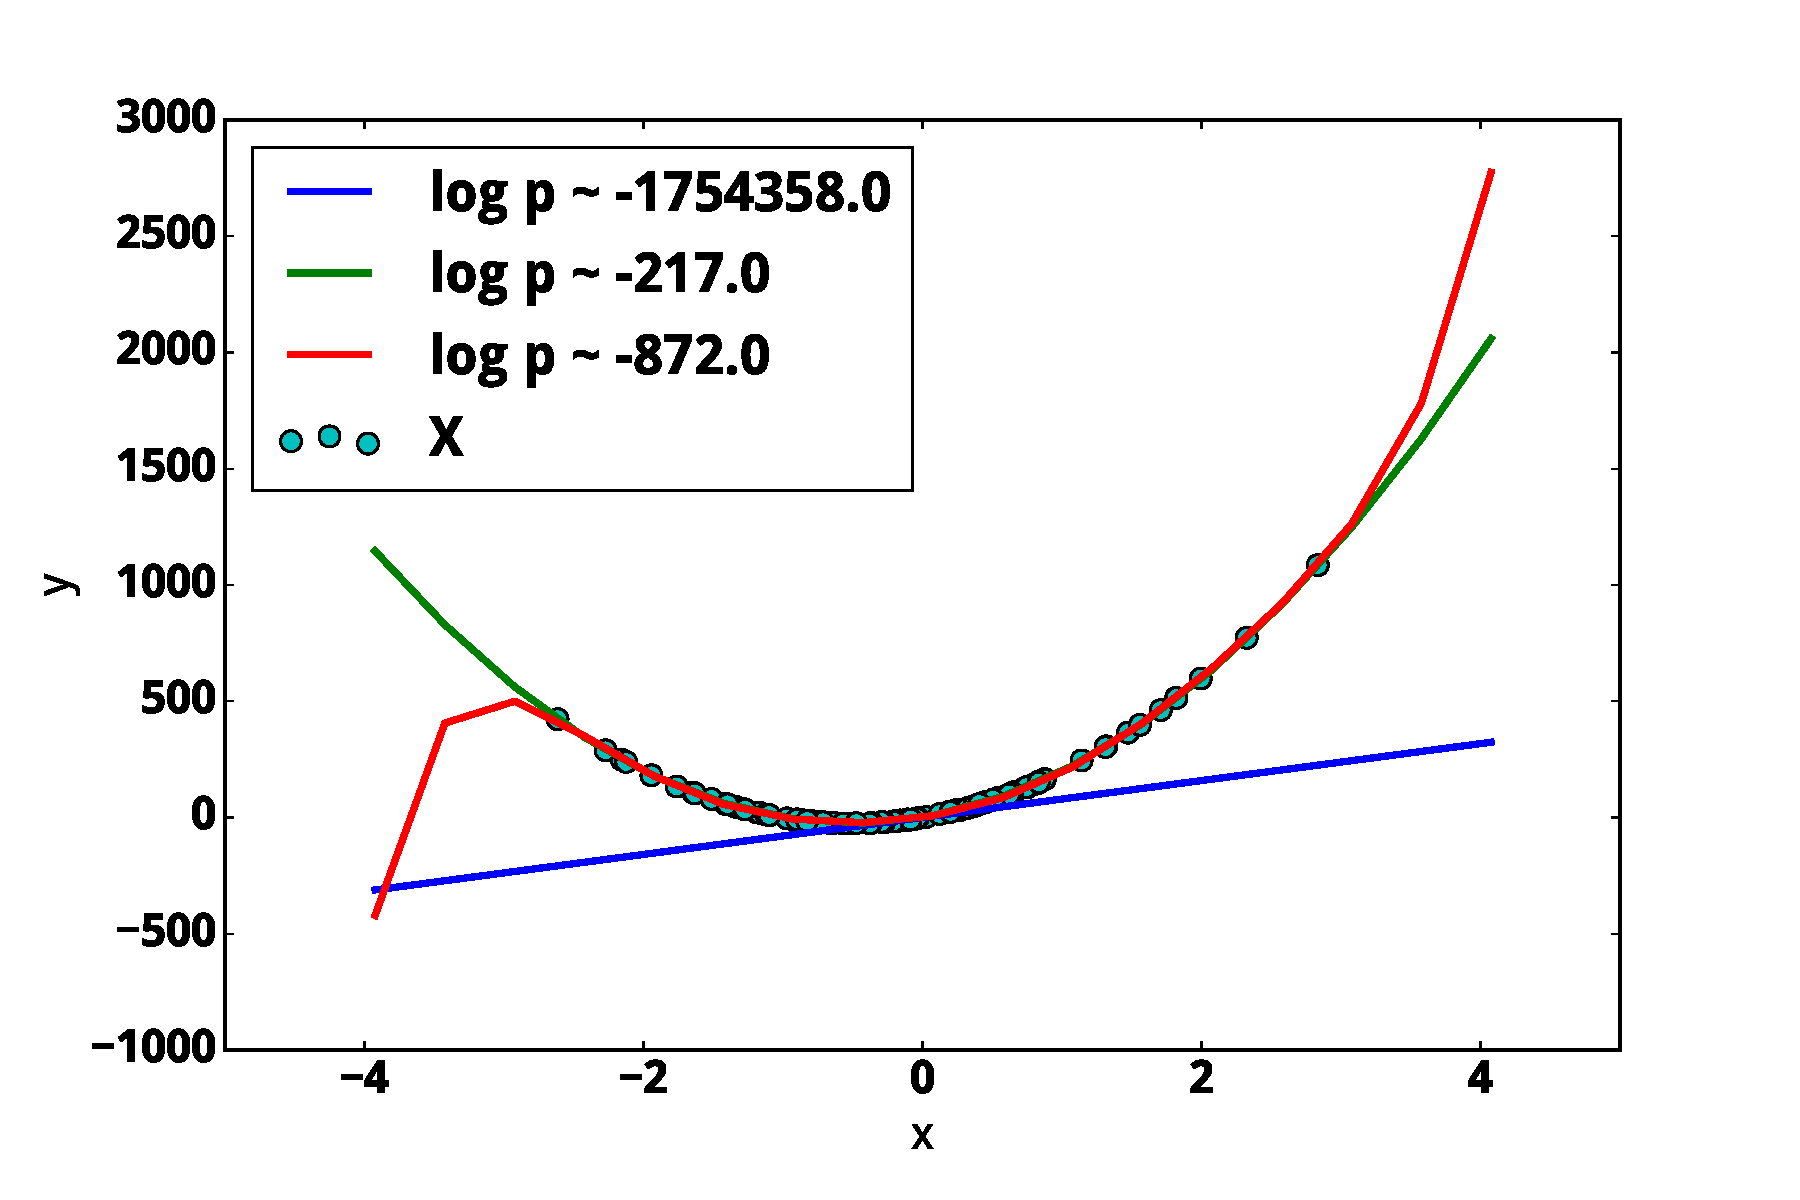
\includegraphics[width=0.35\textwidth]{slide_plots/example.pdf}}

\end{figure}
\end{frame}



\begin{frame}{Выбор оптимальной модели}
\textbf{Основные проблемы выбора оптимальной модели}\\
\begin{itemize}
\item Интеграл правдоподобия $p(\mathbf{y}|\mathbf{X})$ невычислим аналитически.
\item Задача его оптимизации многоэкстремальна и невыпукла.
\end{itemize}
~\\
\textbf{Требуется}\\ 
Предложить метод поиска субоптимального решения задачи оптимизации, обобщающего различные алгоритмы оптимизации:
\begin{itemize}
\item Оптимизация правдоподобия.
\item Последовательное увеличение сложности модели.
\item Последовательное снижение сложности модели.
\item Полный перебор вариантов структуры модели.
\end{itemize}

\end{frame}       


                                                                                                                                   
                                                                                                                                    

\begin{frame}{Вариационная нижняя оценка правдоподобия} 
Интеграл правдоподобия невычислим аналитически.\\
\textbf{Правдоподобие модели:}
\[
p(\mathbf{y}|\mathbf{X}) =
 \int_{\mathbf{W}, \boldsymbol{\Gamma} } \textcolor{red}{p(\mathbf{y}|\mathbf{X},\mathbf{W},  \boldsymbol{\Gamma})} \textcolor{blue}{p(\mathbf{W}, \boldsymbol{\Gamma})}d\mathbf{W}d{\boldsymbol{\Gamma}}.                         
\]

Получим нижнюю оценку интеграла правдоподобия.\\
Пусть $q(\mathbf{W}, \boldsymbol{\Gamma}) = q_{\mathbf{W}}(\mathbf{W})q_{\boldsymbol{\Gamma}}(\boldsymbol{\Gamma})$ --- непрерывное распределение, аппроксимирующее 
апостериорное распределение $p(\mathbf{W}, \boldsymbol{\Gamma}|\mathbf{y}, \mathbf{X})$.
$$                                                                                                                                              
        \text{log}~p(\mathbf{y}|\mathbf{X}) \geq 
\textcolor{blue}{\mathsf{E}_q \text{log}~{p(\mathbf{y} | \mathbf{X}, \mathbf{W}, \boldsymbol{\Gamma})}} - \textcolor{red}{\text{D}_{KL}(p(\mathbf{w}, \boldsymbol{\Gamma}) || q(\mathbf{W}, \boldsymbol{\Gamma}))} = \text{log}\hat{{p}}_{q_{\mathbf{W}}q_{\boldsymbol{\Gamma}}}(\mathbf{y}|\mathbf{X}).
$$ 

Полученная оценка совпадает с интегралом правдоподобия при $$D_\text{KL}(q(\mathbf{W}, \boldsymbol{\Gamma})|(p(\mathbf{W}, \boldsymbol{\Gamma}|\mathbf{y}, \mathbf{X}))=0.$$

\end{frame}      



\begin{frame}
\frametitle{Градиентный спуск как вариационная оценка правдоподобия модели}
\footnotesize

\begin{multicols}{2}

\begin{figure}
\subfloat{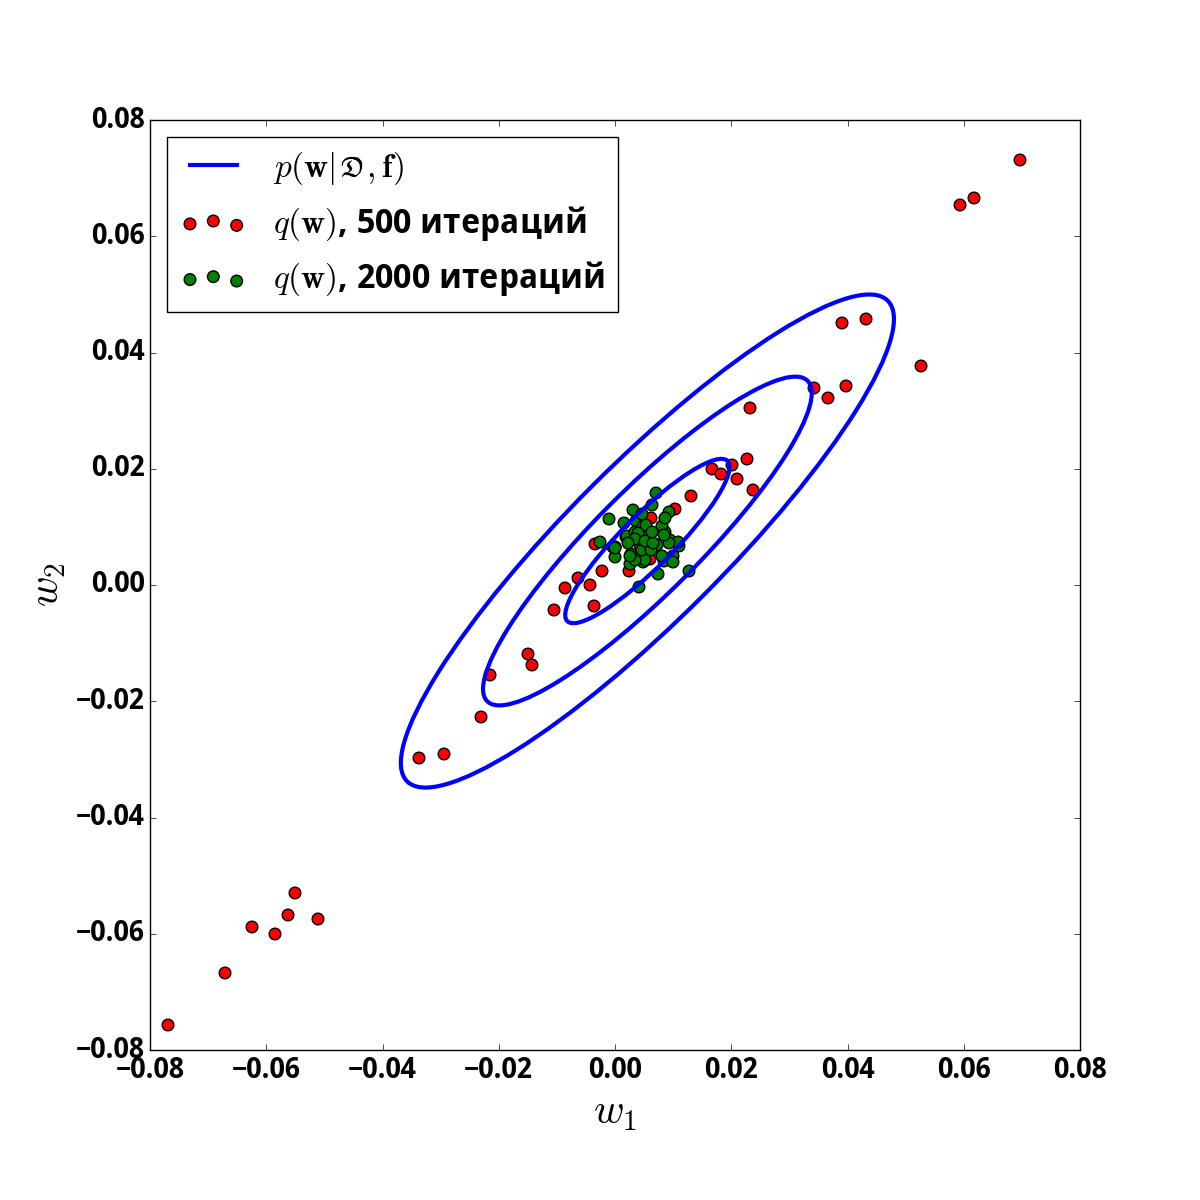
\includegraphics[width=0.38\textwidth]{./slide_plots/sgd_estimate.png}}
\end{figure}

\columnbreak


\begin{figure}
{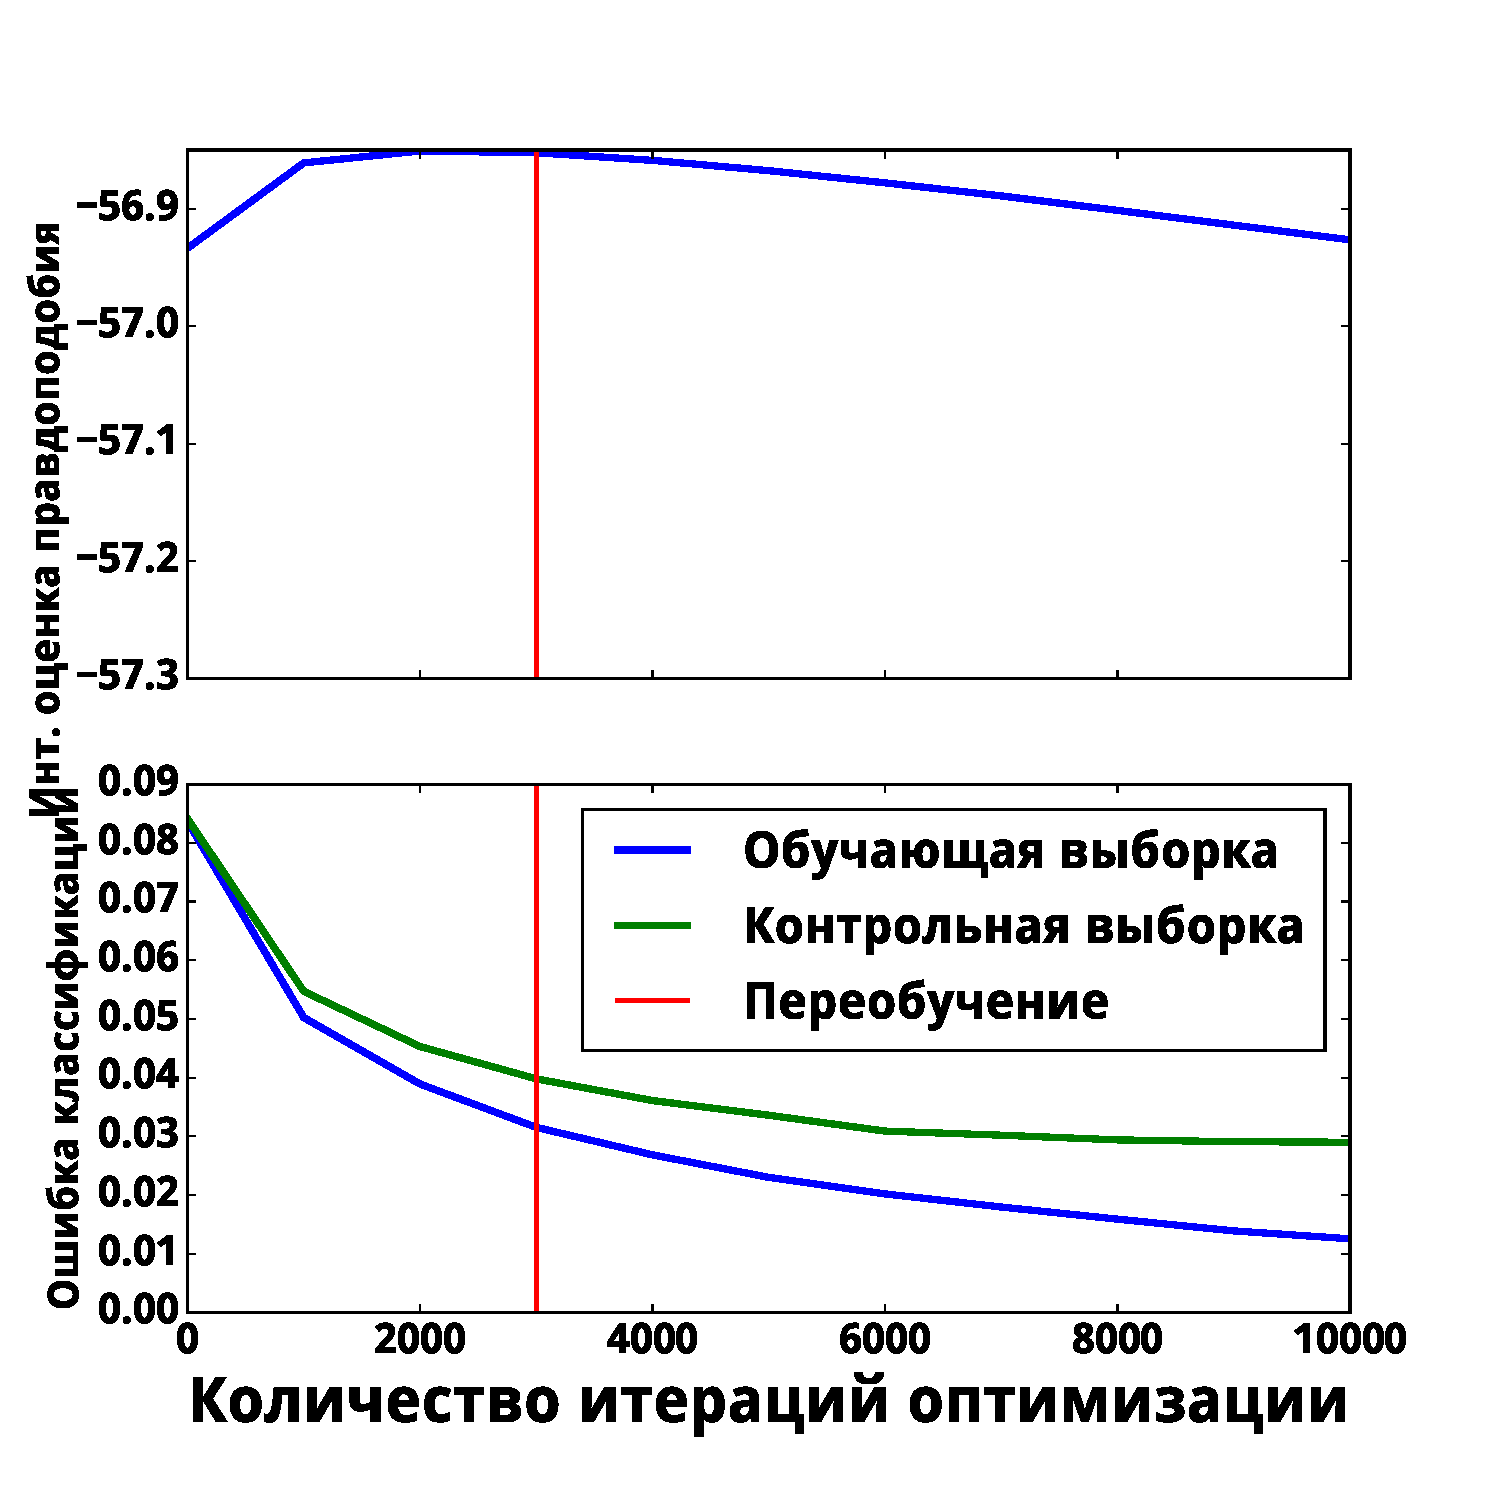
\includegraphics[width=0.38\textwidth]{./slide_plots/sgd_show.pdf}}
\end{figure}
\end{multicols}
\end{frame}


   
\begin{frame}{Выбор вариационного распределения $q$}
\textbf{Вариационное распределение параметров $q_{\mathbf{W}}:$}
$$q_\mathbf{W} = \mathcal{N}(\boldsymbol{\mu}_q, \mathbf{A}^{-1}_q).$$

\textbf{Вариационное распределение структуры $q_{\boldsymbol{\Gamma}}:$}
$$q_{\boldsymbol{\Gamma}}( \mathbf{m}_q, c_\text{temp}) = \prod_{(j,k) \in E} q_{\boldsymbol{\gamma_{j,k}}}(c_\text{temp}, \mathbf{m}_q^{j,k}) \sim \mathcal{GS}(c_\text{temp}, \mathbf{m}_q^{j,k}), \quad |\mathbf{m}_q^{j,k}| = K^{j,k}$$ 
\textbf{Свойства:}
\begin{itemize} 
\item $\lim_{c_\text{temp} \to \infty}  \mathcal{GS}(c_\text{temp}) = \mathcal{U}(\Delta^{K^{j,k} -1}).$
\item При ${c_\text{temp} \to 0}$ распределение вырождается в дискретное распределение.
\item Существует вычислительно устойчивый метод вычисления градиента по параметрам распределения от реализации случайной величины.
\end{itemize}
\end{frame}

\iffalse
\begin{frame}{ Распределение на структуре}
Пусть для каждого ребра $(j,k)$ задан нормированный положительный вектор $\boldsymbol{\gamma}_{j,k} \in \mathbb{R}_{+}^{|K_{j,k}|}$, определяющий веса базовых функций из  $\mathbf{g}(j,k)$.
\\~\\
Будем считать, что вектор $\boldsymbol{\gamma}_{j,k}$ распределен по распределению Gumbel-Softmax($GS$):
\[
    p(\boldsymbol{\gamma}) = (K_{j,k}-1)!{c_{\text{temp}}}^{K_{j,k}-1}\left(\prod_{h=1}^{K_{j,k}-1} \alpha_h \boldsymbol{\gamma}_h^{-c_{\text{temp}}-1}\right)\left(\sum_{h=1}^u\alpha_h\boldsymbol{\gamma}_h^{-c_{\text{temp}}}\right),
\] 
где $\mathbf{m} = [\alpha_1,\dots,\alpha_{K_{j,k}}]$ --- параметры сдвига распределения, $c_{\text{temp}}$ --- температура распределения. 
\\~\\

\end{frame}




\begin{frame}{Вариационный вывод: распределение структурных параметров}
%Для каждого элемента структуры $\boldsymbol{\gamma}$ зададим распределение весов базовых функций по распределению Gumbel-Softmax c параметрами $\hat{\alpha}_1, \dots, \hat{\alpha}_u, c$, где параметр $c$ --- общий для всех весов.

Для реализации $h$-й компоненты случайной величины $\boldsymbol{\gamma}$ справедлива следующая формула:
\[
    \hat{\boldsymbol{\gamma}}^h = \text{exp}\left(\text{log}\left(\alpha_h + \text{Gum}_h\right)c_{\text{temp}}^{-1}\right) \sum_{l=1}^{K_{j,k}} \text{exp}\left(\text{log}\left(\alpha_l + \text{Gum}_l\right)c_{\text{temp}}^{-1}\right),
\]
где $\text{Gum} \sim -\text{log}(-\text{log}~\mathcal{U}(0,1)).$ 

Для всех элементов структуры $\boldsymbol{\gamma}_{j,k}$ положим:
\[
    p(\boldsymbol{\gamma}_{j,k}) = GS([\alpha_1, \dots, \alpha_{K_{j,k}}, c_{\text{temp}}]), \quad q(\boldsymbol{\gamma}_{j,k}) = GS([\hat{\alpha}_1, \dots, \hat{\alpha}_{K_{j,k}}, \hat{c}_{\text{temp}}]),
\]
где $\hat{\alpha}_1, \dots, \hat{\alpha}_{K_{j,k}}, \hat{c}_{\text{temp}}$ --- параметры вариационного распределения.
\end{frame}




    

\begin{frame}{Вариационный вывод: распределение параметров}
Пусть $\mathbf{W} \sim \mathcal{N}(\mathbf{0}, \mathbf{A}^{-1})$ и структура модели $\boldsymbol{\Gamma}$ определена однозначно.

Пусть $q_\mathbf{W} = \mathcal{N}(\boldsymbol{\mu}_q, \mathbf{A}^{-1}_q), \quad \boldsymbol{\theta} =  [\boldsymbol{\mu}_q, \mathbf{A}^{-1}_q].$ \\
Тогда вариационная оценка имеет вид:
$$
\textcolor{blue}{\int_{\mathbf{W}} q(\mathbf{W})\text{log}~{p(\mathfrak{D},\mathbf{W},\mathbf{A}^{-1})} d \mathbf{W}} - \textcolor{red}{D_\text{KL}\bigl(q_\mathbf{W} (\mathbf{W} )|| p (\mathbf{W}|\mathbf{A}^{-1})\bigr)} \simeq
$$
$$
\sum_{i=1}^m \textcolor{blue}{\text{log}~p(\mathbf{x}_i | \mathbf{W}_i)} - \textcolor{red}{D_\text{KL}\bigl(q_\mathbf{W} (\mathbf{W} )|| p (\mathbf{W}|\mathbf{A}^{-1})\bigr)} = -L(\boldsymbol{\theta}, \mathbf{A}^{-1}, \mathfrak{D}),
$$
где $\mathbf{W}_i \sim q_\mathbf{W}$.

Дивергенция $\textcolor{red}{D_\text{KL}\bigl(q_\mathbf{W} (\mathbf{w} )|| p (\mathbf{W}|\mathbf{A}^{-1})\bigr)}$ вычисляется аналитически:
$$
\textcolor{red}{D_\text{KL}\bigl(q_\mathbf{W} (\mathbf{W}) || p (\mathbf{w}|\mathbf{A}^{-1})\bigr)} = \frac{1}{2} \bigl( \text{tr} (\mathbf{A}\mathbf{A}^{-1}_q) + \boldsymbol{\mu}_q^\text{T}\mathbf{A}\boldsymbol{\mu}_q - n +\text{ln}~|\mathbf{A}^{-1}| - \text{ln}~|\mathbf{A}^{-1}_q| \bigr).
$$

\end{frame}

\begin{frame}
\frametitle{Вариационная оценка на основе мультистарта}
$$\text{log}p(\mathbf{y}|\mathbf{X}, \mathbf{A}) \geq \mathsf{E}_{q(\mathbf{W)}}\text{log~}p (\mathbf{y}, \mathbf{W}|\mathbf{X}, \mathbf{A}^{-1}) - \mathsf{E}_{q_{\mathbf{W}}}(-\text{log}(q_\mathbf{W})).$$

\textbf{Теорема [Бахтеев, 2016].}~Пусть $L$ --- функция потерь, градиент которой ---  непрерывно-дифференцируемая функция с константой Липшица $C$. Пусть $\boldsymbol{\theta} = [\mathbf{W}^1,\dots,\mathbf{W}^k]$ ---  начальные приближения оптимизации модели. Пусть $\beta$ --- шаг градиентного спуска, такой что:
\begin{itemize}
\item $\beta<\frac{1}{C}$,
\item $\beta^{(-1)} > \max_{r \in \{1,\dots,k\}}\lambda_\text{max} (\mathbf{H}(\mathbf{W}^r))$.
\end{itemize}
Тогда
\small
\[
	\mathsf{E}_{q^{\tau}_{\mathbf{W}}}(-\text{log}(q^{\tau}_\mathbf{W})) -  \mathsf{E}_{q^{\tau-1}_{\mathbf{W}}}(-\text{log}(q^{\tau-1}_\mathbf{W}))  \sim  \frac{1}{k}\sum_{r=1}^k \bigl(\beta Tr[\mathbf{H}(\mathbf{W}^r)] - \beta^2 Tr[\mathbf{H}(\mathbf{W}^r)\mathbf{H}(\mathbf{w}^r)]  \bigr) + o_{\beta \to 0}(1),
\]
где $\mathbf{H}$ --- гессиан функции потерь $L$, $q^{\tau}_\mathbf{W}$ --- распределение $q^{\tau}_\mathbf{W}$ в момент оптимизации $\tau$.
\end{frame}


\begin{frame}
\frametitle{Вариационная оценка с использованием градиентного спуска}
\footnotesize
Максимизация вариационной оценки эквивалентна минимизации $\text{D}_{\text{KL}}(q(\mathbf{W})||p(\mathbf{W} | \mathfrak{D},\mathbf{A}^{-1}))$.\\
Градиентный спуск не минимизирует $\text{D}_{\text{KL}}(q(\mathbf{W})||p(\mathbf{W} | \mathfrak{D},\mathbf{A}^{-1}))$.
\begin{multicols}{2}

\begin{figure}
\subfloat{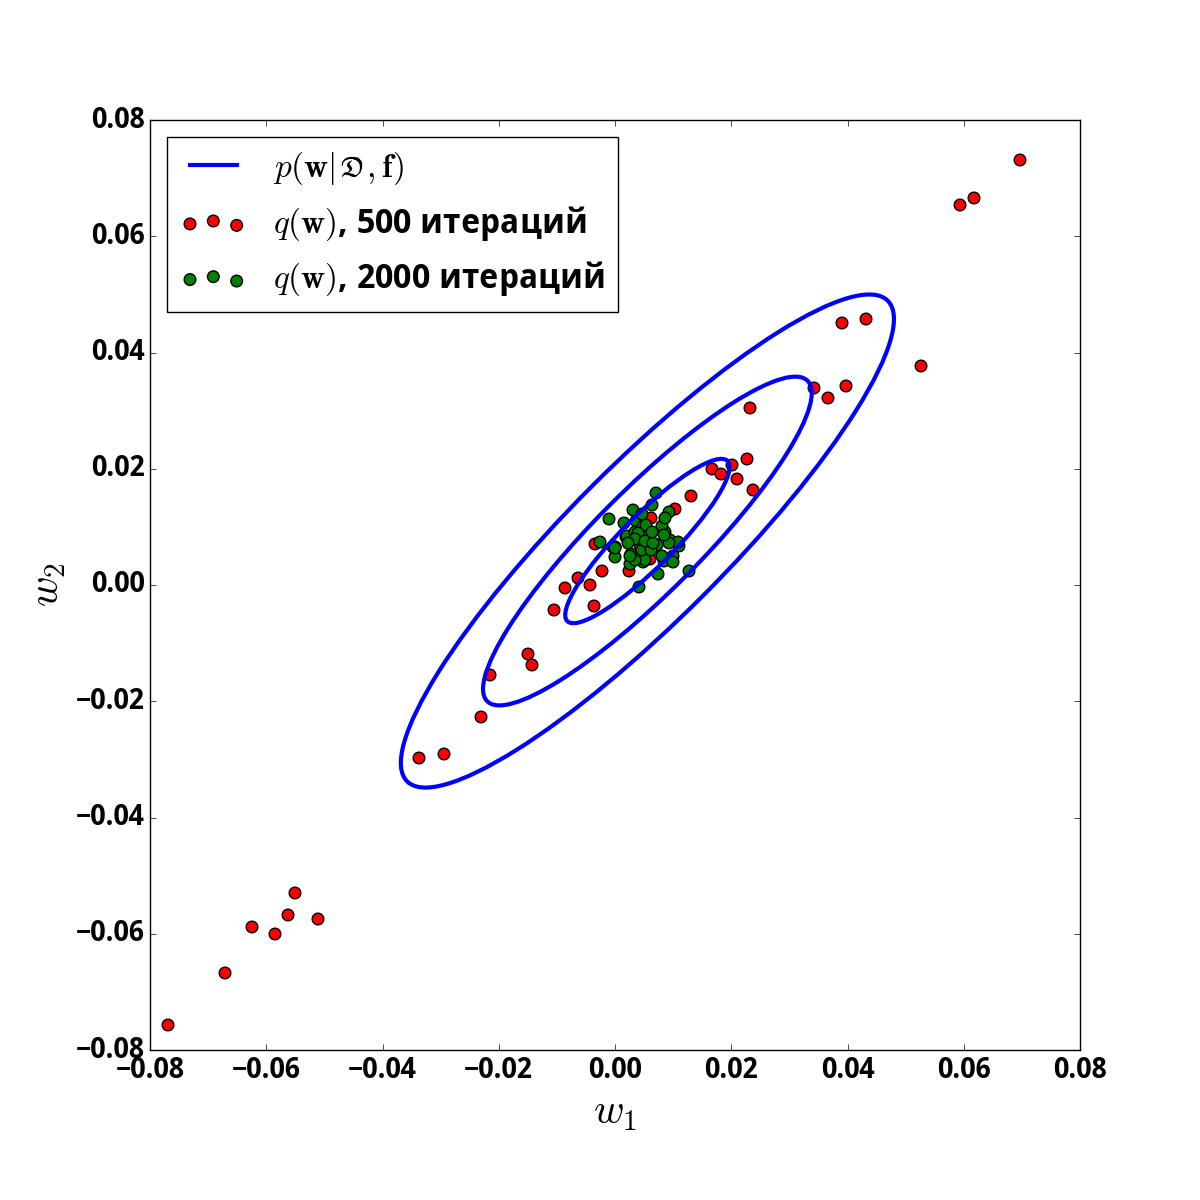
\includegraphics[width=0.38\textwidth]{./slide_plots/sgd_estimate.png}}
\end{figure}

\columnbreak


\begin{figure}
{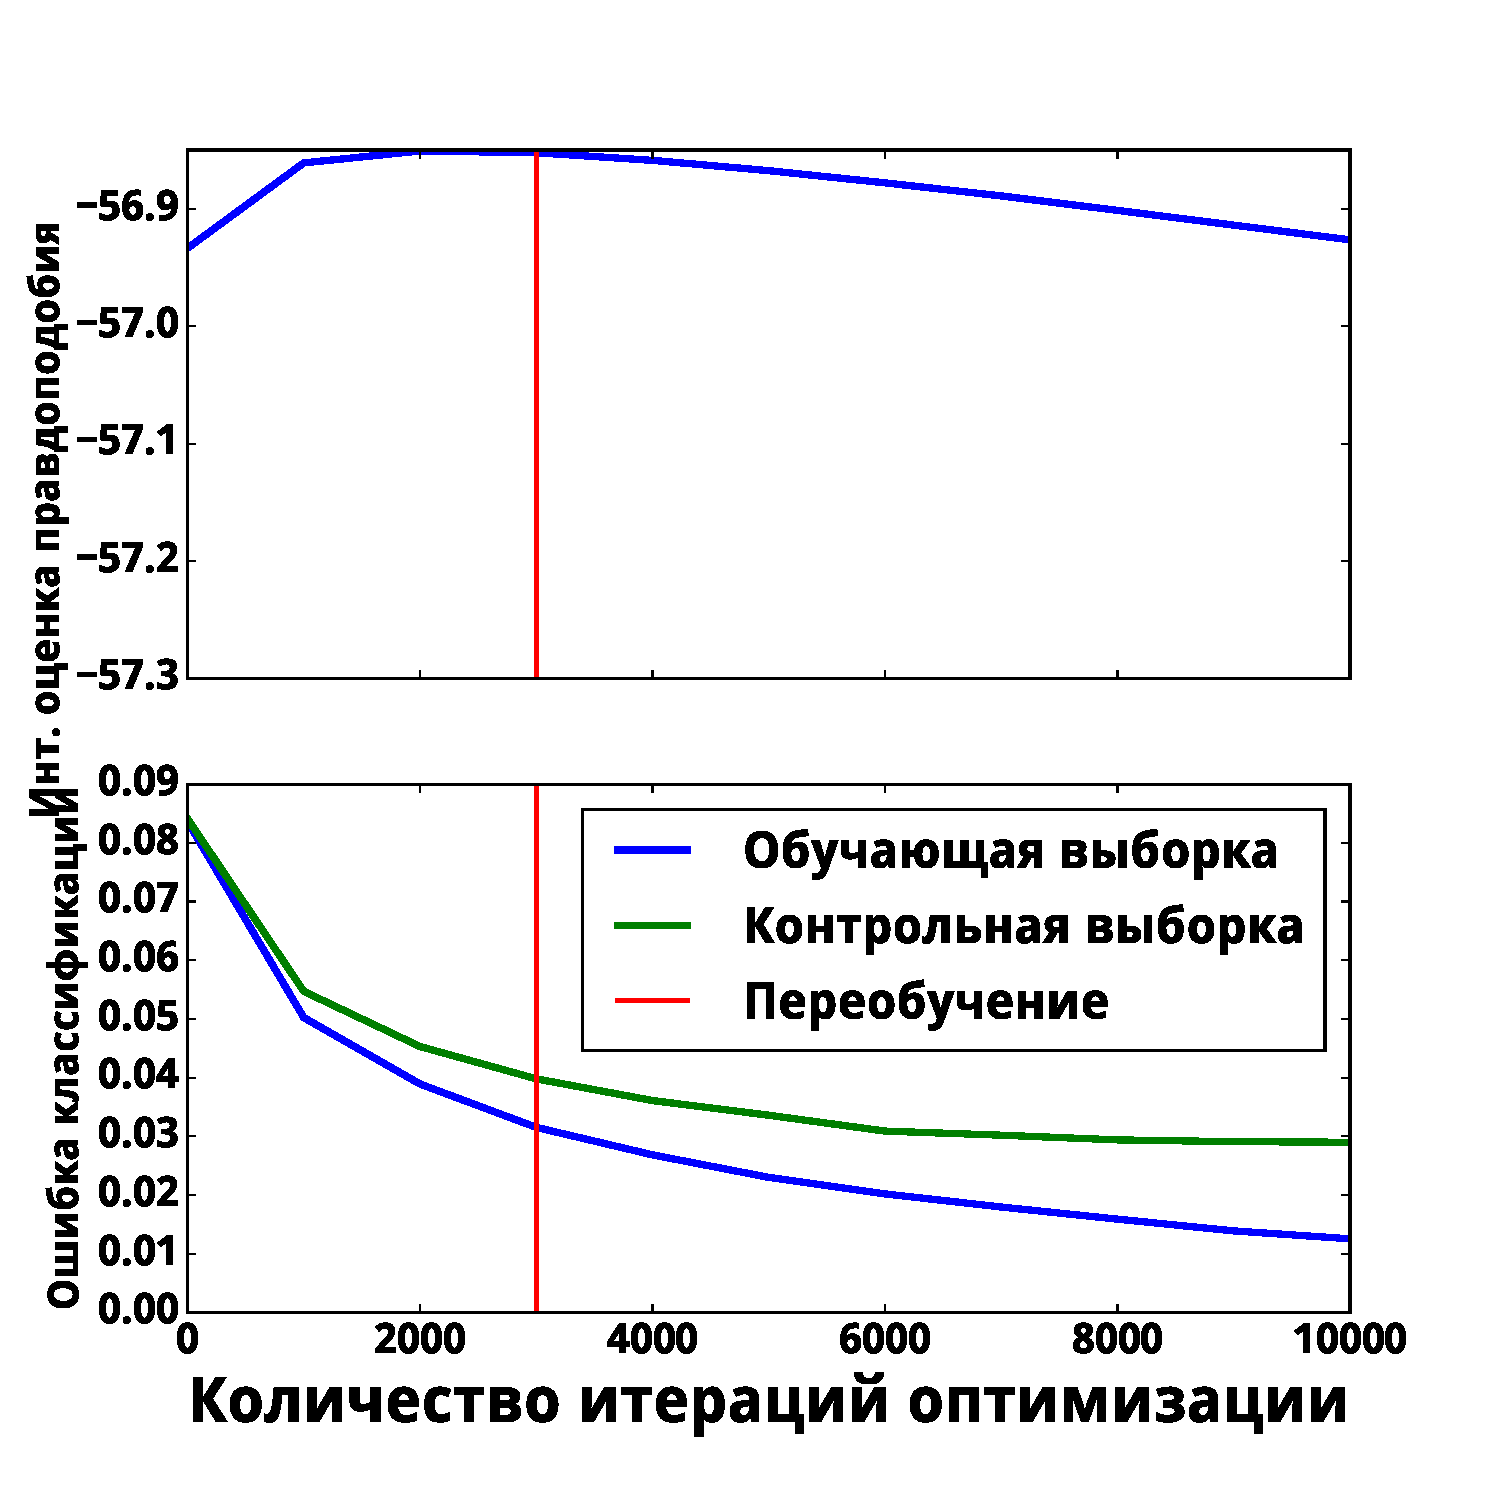
\includegraphics[width=0.38\textwidth]{./slide_plots/sgd_show.pdf}}
\end{figure}
\end{multicols}
\end{frame}

\fi 

\begin{frame}{Оптимизация параметров вариационного распределения}
\footnotesize
Параметры вариационного распределения $q(\mathbf{W}, \boldsymbol{\Gamma}) = q_{\mathbf{W}}(\mathbf{W})q_{\boldsymbol{\Gamma}}(\boldsymbol{\Gamma})$ оптимизируем:
\[
L =
\textcolor{blue}{\mathsf{E}_q \text{log}~{p(\mathbf{y} | \mathbf{X}, \mathbf{W}, \boldsymbol{\Gamma}. \mathbf{A}^{-1}, c_{\text{temp}})}} - \textcolor{red}{c_\text{reg}\text{D}_{KL}\left(p(\mathbf{w}, \boldsymbol{\Gamma} |\mathbf{A}^{-1}, \mathbf{m}, c_{\text{temp}}) || q(\mathbf{W}), q(\boldsymbol{\Gamma})\right)} \to \max_{\mathbf{A}_q, \boldsymbol{\mu}_q, \mathbf{m}_q}
\]

\begin{block}{Теорема [Бахтеев, 2018].}
Пусть $c_\text{reg} > 0$ .
Тогда функция $L$ сходится по вероятности к вариационной нижней оценке логарифма правдоподобия $\text{log}~p(\mathbf{y}|\mathbf{x})$ для случайной подвыборки  $\mathfrak{D}$ 
мощностью $c_\text{reg} m$:
$$
L \to^p c_\text{reg} m \text{log}\hat{{p}}_{q_{\mathbf{W}}q_{\boldsymbol{\Gamma}}}(\mathbf{y}|\mathbf{X}).
$$
\end{block}

\begin{block}{Теорема  [Бахтеев, 2018].}
Для любых значений $\mathbf{A}, \mathbf{m}$ и вариационных параметров $\boldsymbol{\mu}_q, \mathbf{A}_q$ существует такая точка $\mathbf{m}_q^1$ на вершинах симплексов структуры $\boldsymbol{\Gamma}$,  что для любой точки  $\mathbf{m}_q^2$ внутри симплексов справедливо выражение:
$$\lim_{c_\text{temp} \to 0}\frac{\text{log}\hat{{p}}_{q_{\mathbf{W}}q^2_{\boldsymbol{\Gamma}}}(\mathbf{y}|\mathbf{X})}{\text{log}\hat{{p}}_{q_{\mathbf{W}}q_{\boldsymbol{\Gamma}}}(\mathbf{y}|\mathbf{X})} = -\infty,\text{\quad где}
q_{\boldsymbol{\Gamma}}^1 = q_{\boldsymbol{\Gamma}}( \mathbf{m}_q^1, c_\text{temp}), \quad q_{\boldsymbol{\Gamma}}^2 = q_{\boldsymbol{\Gamma}}^1(\mathbf{m}_q^2, c_\text{temp})).$$
\end{block}
\end{frame}


\begin{frame}{Оптимизация параметров априорного распределения}
Гиперпараметры $\mathbf{A}, \mathbf{m}$ оптимизируем:
\[
Q = \textcolor{blue}{c_\text{train}\mathsf{E}_q \text{log}~{p(\mathbf{y} | \mathbf{X}, \mathbf{W}, \boldsymbol{\Gamma}. \mathbf{A}^{-1}, c_{\text{prior}})}}
 - \textcolor{red}{c_\text{prior}\text{D}_{KL}(p(\mathbf{W}, \boldsymbol{\Gamma} |\mathbf{A}^{-1}, \mathbf{m}, c_{\text{temp}}) || q(\mathbf{W}, \boldsymbol{\Gamma}))} -\]
\[
 - \textcolor{OliveGreen}{c_{\text{comb}}\sum_{p' \in \mathbf{P}} \text{D}_{KL}(\boldsymbol{\Gamma} | p')} \to \max, 
\]
где $\mathbf{P}$ --- множество (возможно пустое) распределений на структуре модели.
\begin{itemize}
\item $\textcolor{blue}{c_\text{train}}$ --- коэффициент правдоподобия выборки;
\item $\textcolor{red}{c_\text{prior}}$ --- коэффициент регуляризации модели;
\item $\textcolor{OliveGreen}{c_{\text{comb}}}$ --- коэффициент перебора структуры.
\end{itemize}
\end{frame}

\begin{frame}{Общая задача оптимизации}
Общая задача оптимизации --- двухуровневая:
\[
\hat{\mathbf{A}}, \hat{\mathbf{m}} = \argmax_{\mathbf{A}, \mathbf{m}} Q = 
\]
\[
= \textcolor{blue}{c_\text{train}\mathsf{E}_{\hat{q}} \text{log}~{p(\mathbf{y} | \mathbf{X}, \mathbf{W}, \boldsymbol{\Gamma}. \mathbf{A}^{-1}, c_{\text{prior}})}}
 - \textcolor{red}{c_\text{prior}\text{D}_{KL}(p(\mathbf{W}, \boldsymbol{\Gamma} |\mathbf{A}^{-1}, \mathbf{m}, c_{\text{temp}}) || \hat{q}(\mathbf{W}, \boldsymbol{\Gamma}))} -\]
\[
 - \textcolor{OliveGreen}{c_{\text{comb}}\sum_{p' \in \mathbf{P}} \text{D}_{KL}(\boldsymbol{\Gamma} | p')}, 
\]
где 
\[
\hat{q} = \argmax_{q} L = 
\textcolor{blue}{\mathsf{E}_q \text{log}~{p(\mathbf{y} | \mathbf{X}, \mathbf{W}, \boldsymbol{\Gamma}. \mathbf{A}^{-1}, c_{\text{temp}})}} - \textcolor{red}{c_\text{reg}\text{D}_{KL}(p(\mathbf{w}, \boldsymbol{\Gamma} |\mathbf{A}^{-1}, \mathbf{m}, c_{\text{temp}}) || q(\mathbf{W}), q(\boldsymbol{\Gamma}))}
\]

\end{frame}


\begin{frame}{Оператор оптимизации}
\small
Обозначим за $\mathbf{h}$ гиперпараметры $\mathbf{A}, \mathbf{m}$.\\
Обозначим за $\boldsymbol{\theta}$ параметры распределений $q_{\mathbf{W}}, q_{\boldsymbol{\Gamma}}$.

\begin{block}{Определение}
Оператором $T$ назовем оператор стохастического градиентного спуска, производящий $\eta$ шагов оптимизации:
\[
	 \hat{\boldsymbol{\theta}} = T \circ T \circ \dots \circ T(\boldsymbol{\theta}_0, \mathbf{A}^{-1}) = T^\eta(\boldsymbol{\theta}_0, \mathbf{A}^{-1}), \quad\text{где}	T(\boldsymbol{\theta}, \mathbf{A}^{-1}) =\boldsymbol{\theta} - \beta \nabla L(\boldsymbol{\theta}, \mathbf{A}^{-1})|_{\hat{\mathfrak{D}}}, 
\]
$\gamma$ --- длина шага градиентного спуска, $\boldsymbol{\theta}_0$ --- начальное значение параметров $\boldsymbol{\theta}$, $\hat{\mathfrak{D}}$ --- случайная подвыборка исходной выборки $\mathfrak{D}$.
\end{block}

Перепишем итоговую задачу оптимизации:
\[
	\hat{\mathbf{h}} = \argmax_{\mathbf{h}} Q( T^\eta(\boldsymbol{\theta}_0, \mathbf{A}^{-1})),
\]
где $\boldsymbol{\theta}_0$ --- начальное значение $\boldsymbol{\theta}$.



\end{frame}




\iffalse
\begin{frame}{Оптимизация гиперпараметров}



\begin{block}{Утверждение, Luketina et al., 2016}
Пусть функции $L$ и $Q$ являются дважды дифференцируемыми и выпуклыми. 
Пусть гессиан функции функции $L$ аппроксимируется единичной матрицей:
\[
    \mathbf{H}(L, \boldsymbol{\theta}) \approx \mathbf{I}.
\]
Тогда допустима следующая оптимизация гиперпараметров:
\[
    \mathbf{h}' = \mathbf{h} - \beta^{h} \nabla_{\mathbf{h}} Q(T(\boldsymbol{\theta}), \mathbf{h}),
\]
где $\beta^{h}$ --- шаг оптимизации гиперпараметров.
\end{block}
\end{frame}

\fi 

\begin{frame}{Оптимизация гиперпараметров: пример}
\begin{multicols}{2}
\begin{figure}[h]
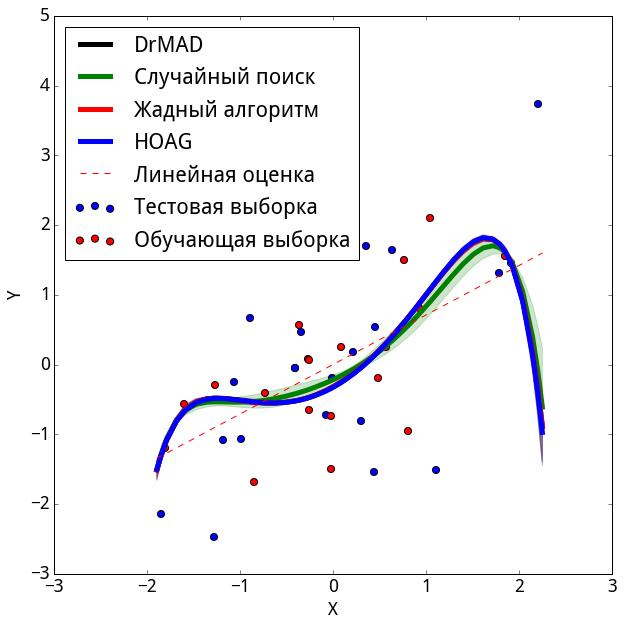
\includegraphics[width=0.4\textwidth]{./slide_plots/poly_cv.png}
\caption*{Кросс-Валидация}
\end{figure}

\begin{figure}[h]
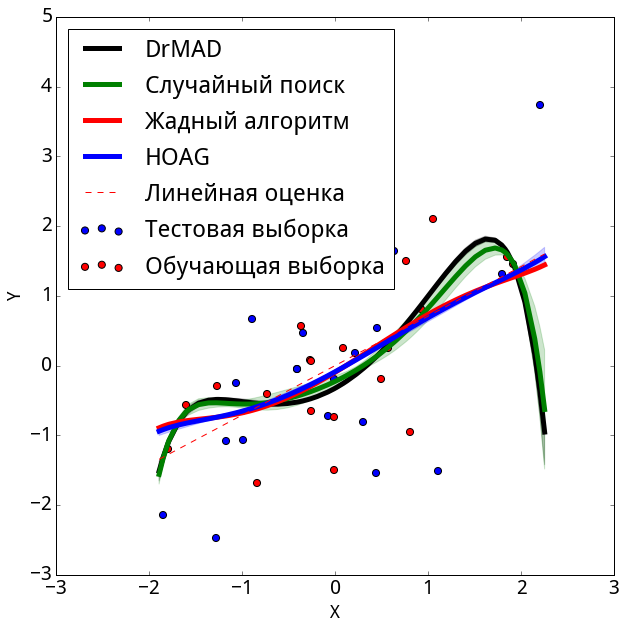
\includegraphics[width=0.4\textwidth]{./slide_plots/poly_var.png}
\caption*{Вариационная оценка}
\end{figure}
\end{multicols}

\end{frame}

\begin{frame}{Оптимизация правдоподобия модели}
\begin{block}{Теорема  [Бахтеев, 2018].}
Пусть существуют параметры распределения $q(\mathbf{W}, \boldsymbol{\Gamma})$, такие что $\text{D}_\text{KL}(q(\mathbf{W}, \boldsymbol{\Gamma})|p(\mathbf{W},  \boldsymbol{\Gamma}| \mathbf{y}, \mathbf{X}, \mathbf{A}, \mathbf{m}, c_\text{temp})) = 0$.\\
Тогда двухуровневая задача оптимизация эквивалентна задаче оптимизации правдоподобия модели:
$$\argmax_{\mathbf{A}, \mathbf{m}}  p(\mathbf{y}|\mathbf{X},\mathbf{A},\mathbf{m}, c_{\text{temp}})$$ 
при $c_{\text{reg}} = c_{\text{prior}} = c_{\text{train}} >0, c_{\text{comb}} = 0$. 
\end{block}
~\\

\end{frame}

\begin{frame}{Параметрическая сложность}
\small
Обозначим за $F(c_{\text{reg}}, c_{\text{train}}, c_{\text{prior}}, c_{\text{comb}}, \mathbf{P}, c_{\text{temp}})$ множество экстремумов функции $L$ при решении задачи двухуровневой оптимизации.
\begin{block}{Теорема [Бахтеев, 2018].}
Пусть $\mathbf{f} \in F(1, 1, c_{\text{prior}}, 0, \{\},  c_{\text{temp}} )$.
При устремлении $ c_{\text{prior}}$ к бесконечности параметрическая сложность модели $\mathbf{f}$ устремляется к нулю.
\[
    \lim_{c_{\text{prior}} \to \infty} C_{\text{param}}(\mathbf{f}) = 0
\]
\end{block}

\begin{block}{Теорема [Бахтеев, 2018].}
Пусть $\mathbf{f}_1 \in F(1, 1, c_{\text{prior}}^1, 0, \{\},  c_{\text{temp}} ), \mathbf{f}_2 \in F(1, 1, c_{\text{prior}}^2, 0, \{\},  c_{\text{temp}})$, $c_{\text{prior}}^1 < c_{\text{prior}}^2$.\\
Пусть вариационные параметры моделей $\mathbf{f}_1$ и $\mathbf{f}_2$ лежат в области $\mathsf{U}$, в которой соответствующие функции $L$ и $Q$ являются локально-выпуклыми.\\ 
Тогда модель $\mathbf{f}_1$ имеет параметрическую сложность, не меньшую чем у $\mathbf{f}_2$.
\[
    C_\text{param}(\mathbf{f}_1) \geq C_\text{param}(\mathbf{f}_2).
\]
\end{block}


\end{frame}

\begin{frame}{Структурная сложность}
\small

\begin{block}{Теорема  [Бахтеев, 2018].}
Пусть для каждого ребра $(i,j)$ семейства моделей $\mathfrak{F}$ априорное распределение $$p(\boldsymbol{\gamma}_{i,j}) =  \lim_{c_{\text{temp}} \to 0} \mathcal{GS}(c_{\text{temp}}).$$
Пусть $c_{\text{reg}} >0, c_{\text{train}} >0, c_{\text{prior}}>0$.
Пусть $\mathbf{f} \in F(c_{\text{reg}}, c_{\text{train}}, c_{\text{prior}}, 0, \{\}, c_{\text{temp}})$.
Тогда структурная сложность модели $\mathbf{f}$ равняется нулю.
\[
    C_\text{struct}(\mathbf{f}) = 0
\]
\end{block}

\begin{block}{Теорема [Бахтеев, 2018].}
Пусть $\mathbf{f}_1 \in F(c_{\text{reg}}, c_{\text{train}},  c_{\text{prior}}, 0, \{\},  c^1_{\text{temp}}), \mathbf{f}_2 =  \in \lim_{c^2_{\text{temp}} \to \infty} F(c_{\text{reg}}, c_{\text{train}},  c_{\text{prior}}, 0, \{\},  c^2_{\text{temp}})$.
Пусть вариационные параметры моделей $f_1$ и $f_2$ лежат в области $U$, в которой соответствующие функции $L$ и $Q$ являются локально-выпуклыми. 
Тогда разница структурных сложностей моделей ограничена выражением:
\[
    C_\text{struct}(\mathbf{f}_1)  - C_\text{struct}(\mathbf{f}_2) \leq \textcolor{blue}{\mathsf{E}_q^1 \text{log}~{p(\mathbf{y} | \mathbf{X}, \mathbf{W}, \boldsymbol{\Gamma}. \mathbf{A}^{-1}, c^1_{\text{temp}})}} - \textcolor{blue}{\mathsf{E}_q^2 \text{log}~{p(\mathbf{y} | \mathbf{X}, \mathbf{W}, \boldsymbol{\Gamma}, \mathbf{A}^{-1})}}.
\]
\end{block}

% Схема доказательства:
% расписываем неравенства вида: L_1 - DKL(q_1|p1) <L_2 - DKL(q_2|p1)
% Замечаем, что при стремлении к бесконечности гумбель превращается в равномерное
% выражаем все в равномерном
% замечаем, что D_KL = Entropy + const для равномерного
% все
\end{frame}


\begin{frame}{Полный перебор}
\small
Пусть для каждого ребра $(i,j)$ семейства моделей $\mathfrak{F}$ априорное распределение $$p(\boldsymbol{\gamma}_{i,j}) =  lim_{c_{\text{temp}} \to 0} \mathcal{GS}(c_{\text{temp}}).$$

Рассмотрим последовательность $N = \prod_{(j,k) \in E} K_{j,k}$ моделей, полученных в ходе оптимизаций вида:
$$f_1 \in F(c_{\text{reg}}, 0, 0, \{\}, c_{\text{comb}},  c_{\text{temp}}),$$
$$f_2 \in F(c_{\text{reg}}, 0, 0, \{q_1(\boldsymbol{\Gamma})\},  c_{\text{comb}},  c_{\text{temp}}),$$
$$f_3 \in F(c_{\text{reg}}, 0, 0, \{q_1(\boldsymbol{\Gamma}), q_2(\boldsymbol{\Gamma})\},  c_{\text{comb}},  c_{\text{temp}}),$$
где $C_{\text{reg}} > 0,  c_{\text{comb}}>0$.


\begin{block}{Теорема}
Вариационные распределения структур $q_{\boldsymbol{\Gamma}}$ последовательности вырождаются в распределения вида $\delta(\hat{\mathbf{m}})$, где $\hat{\mathbf{m}}$ --- точка на декартовом произведении вершин симплексов структуры модели.

Последовательность соответствует полному перебору структуры $\boldsymbol{\Gamma}$.
\end{block}
\end{frame}


\begin{frame}{Заключение}
\begin{itemize}
\item Предложен алгоритм оптимизации параметров, гиперпараметров и структурных
параметров моделей глубокого обучения.
\item Предложен метод выбора модели наиболее правдоподобной структуры, обобщающий различные алгоритмы оптимизации:
\begin{itemize}
\item оптимизация правдоподобия;
\item последовательное увеличение сложности модели;
\item последовательное снижение сложности модели;
\item полный перебор вариантов структуры модели.
\end{itemize}
\item Проведено исследование свойства оптимизационных алгоритмов выбора модели.

\end{itemize}
\end{frame}







\end{document}
